\documentclass[12pt]{article}
\usepackage{graphicx}
\usepackage{hyperref}
\usepackage[a4paper, total={6in, 8in}]{geometry}
\usepackage{setspace}
\usepackage{parskip}
\usepackage{tabularx}
\usepackage{multirow}
\usepackage{booktabs}
\usepackage{amsmath}
\usepackage{listings}
\usepackage{xcolor}
\usepackage{float}
\usepackage{longtable}
\usepackage{fancyvrb}

\linespread{1.1}

\lstset{
  basicstyle=\ttfamily\small,
  keywordstyle=\color{blue},
  commentstyle=\color{gray},
  stringstyle=\color{red},
  breaklines=true,
  frame=single,
  numbers=left,
  numberstyle=\tiny\color{gray}
}

\title{SEC-EDGAR-GPT: A 124M Financial Language Model%
\thanks{Code: \url{https://github.com/lzwjava/sec-edgar-gpt} \quad
Model: \url{https://huggingface.co/lzwjava/sec-edgar-gpt-124m-hf}}}
\author{
  Zhiwei Li\thanks{Independent Researcher. Email: lzwjava@gmail.com.}
}
\date{June 2026}

\begin{document}

\maketitle

\begin{abstract}
We present a 124-million parameter GPT-2 language model trained on 1.55 billion tokens of SEC-EDGAR financial filings using the nanoGPT framework. The model was trained on a single NVIDIA RTX 4070 GPU over approximately 8 hours, training for the full 47,000 steps and converging to a final validation loss of 2.28. We evaluate the model's generation quality across multiple SEC filing sections including business descriptions, management discussion and analysis, risk factors, financial notes, and proxy statements. Our analysis reveals that the model successfully learns SEC document structure, financial vocabulary, and boilerplate language patterns, but exhibits characteristic limitations in long-range coherence, numerical consistency, and table extension. We present extensive generation samples demonstrating both the strengths and failure modes of small domain-specific language models. We discuss the implications for using small language models in financial document generation and the trade-offs between model size, training data quality, and generation fidelity.
\end{abstract}

\section{Introduction}

The proliferation of large language models (LLMs) has created significant interest in domain-specific text generation. Financial filings submitted to the U.S. Securities and Exchange Commission (SEC) through the EDGAR system represent a particularly rich corpus of structured, domain-specific text. These documents follow strict formatting conventions and employ specialized financial vocabulary, making them an interesting testbed for evaluating language model capabilities in structured document generation.

While state-of-the-art models like GPT-4 and Claude demonstrate impressive general-purpose capabilities, the cost and computational requirements of training and deploying such models limit their accessibility. In this work, we investigate whether a smaller, more accessible model---a 124M parameter GPT-2---can learn to generate convincing SEC filing text when trained on a focused corpus of EDGAR documents.

Our contributions include:
\begin{itemize}
    \item Training a 124M parameter GPT-2 model on 1.55 billion tokens of SEC-EDGAR filings using consumer hardware (RTX 4070, 12GB VRAM)
    \item Detailed training loss analysis showing convergence from 10.98 to 2.28 validation loss
    \item Systematic evaluation of generation quality across five distinct SEC filing sections with extensive samples
    \item Analysis of long-range coherence, numerical consistency, and structural fidelity
    \item Discussion of practical applications and limitations for financial document generation
\end{itemize}

\section{Related Work}

\subsection{Language Models for Financial Text}

Recent work has explored applying language models to financial domains. BloombergGPT \cite{bloomberggpt} trained a 50B parameter model on a mixed corpus including financial data. FinGPT \cite{fingpt} proposed open-source financial language models. However, these efforts focused on much larger models and broader financial tasks.

\subsection{Small Language Models}

The original GPT-2 \cite{gpt2} demonstrated that language models could generate coherent text at various scales (124M to 1.5B parameters). More recent work has shown that smaller models can achieve surprising performance when trained on high-quality, domain-specific data \cite{tinystories}.

\subsection{SEC-EDGAR as Training Data}

The SEC-EDGAR database contains millions of corporate filings spanning decades. Prior work has used EDGAR data for sentiment analysis \cite{edgar-sentiment} and information extraction \cite{edgar-extraction}, but little work has explored using EDGAR as a primary training corpus for generative language models.

\section{Methodology}

\subsection{Data Collection and Preparation}

We collected SEC-EDGAR filings from the CodeParrot GitHub dataset, which contains processed EDGAR documents. The training corpus consists of:

\begin{table}[H]
\centering
\begin{tabular}{lr}
\toprule
\textbf{Metric} & \textbf{Value} \\
\midrule
Total training tokens & 1.55B \\
Number of training shards & 16 \\
Validation tokens & 100M \\
Average document length & ~2,048 tokens \\
Vocabulary & GPT-2 BPE (50,257 tokens) \\
\bottomrule
\end{tabular}
\caption{SEC-EDGAR training corpus statistics}
\label{tab:corpus}
\end{table}

The data was tokenized using the GPT-2 byte-pair encoding tokenizer and stored as memory-mapped numpy arrays for efficient training.

\subsection{Model Architecture}

We use the standard GPT-2 architecture with the following configuration:

\begin{table}[H]
\centering
\begin{tabular}{lr}
\toprule
\textbf{Parameter} & \textbf{Value} \\
\midrule
Number of layers & 12 \\
Number of attention heads & 12 \\
Embedding dimension & 768 \\
Context length & 1,024 tokens \\
Total parameters & 123.59M \\
Vocabulary size & 50,257 \\
\bottomrule
\end{tabular}
\caption{GPT-2 124M model configuration}
\label{tab:model}
\end{table}

\subsection{Training Setup}

Training was conducted on a single NVIDIA RTX 4070 GPU with 12GB VRAM using the nanoGPT framework. 

\begin{figure}[H]
\centering
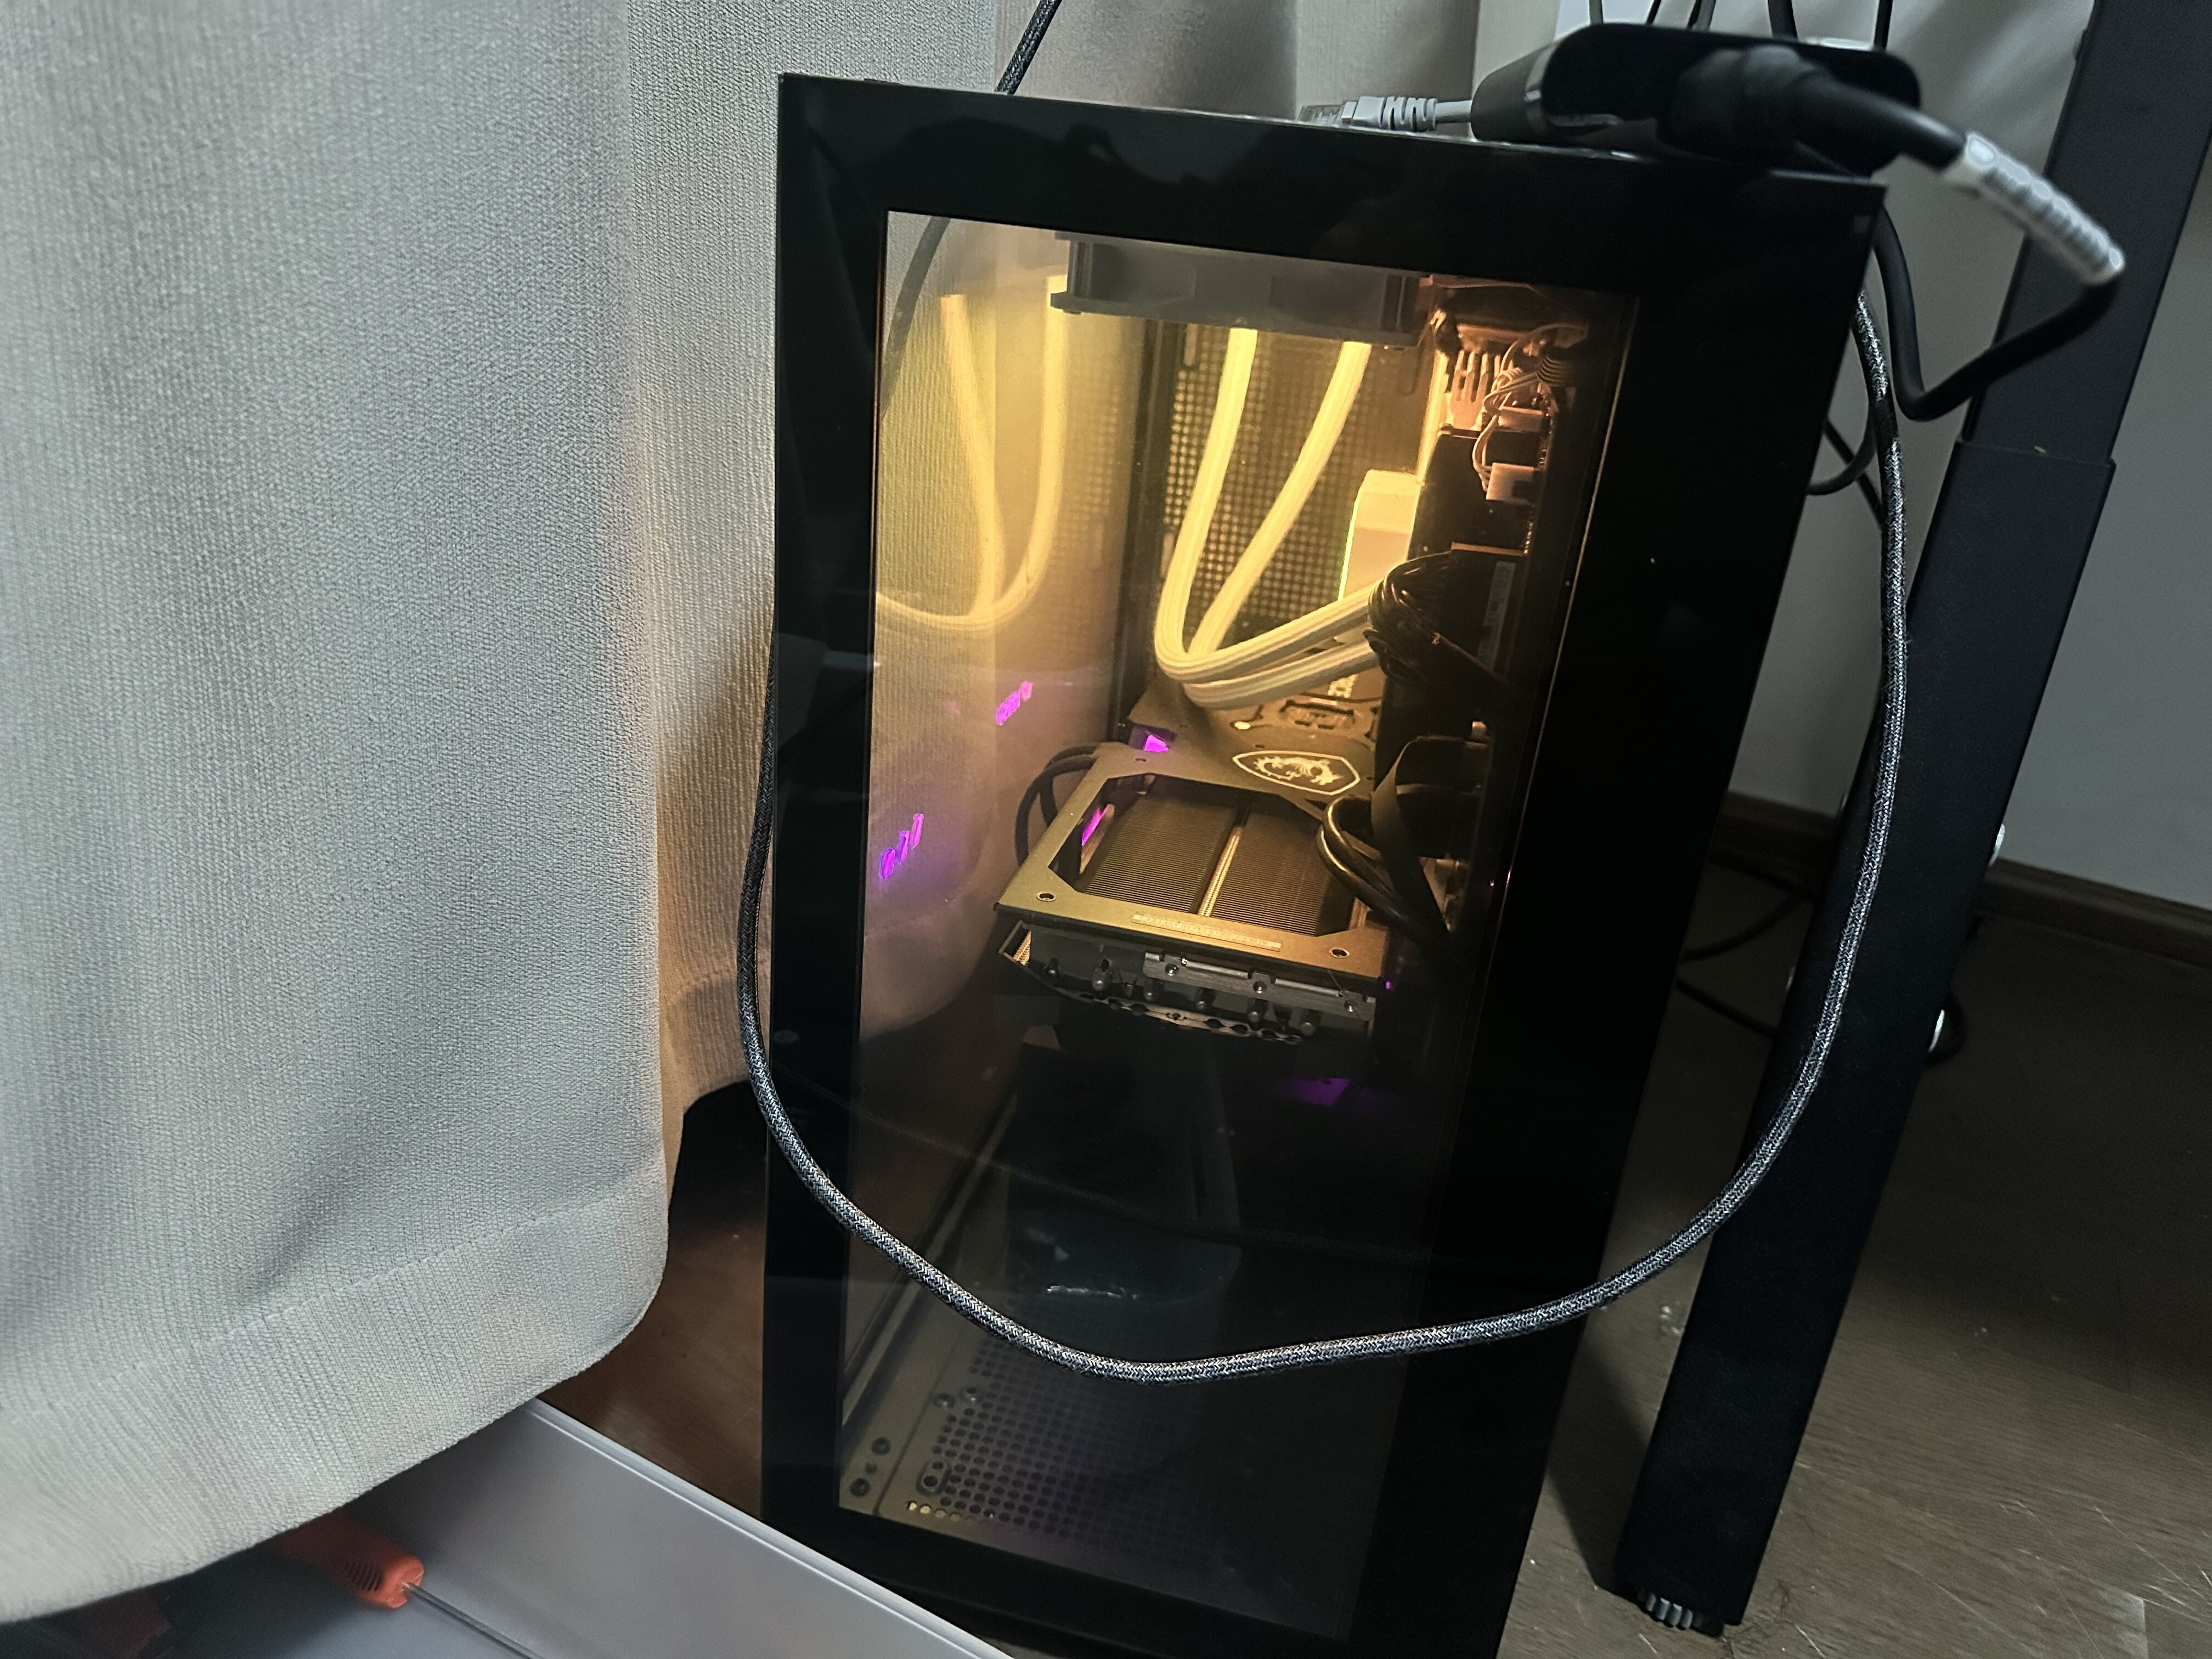
\includegraphics[width=\textwidth]{paper4.jpg}
\caption{Training workstation equipped with NVIDIA RTX 4070 GPU used for all experiments in this paper.}
\label{fig:workstation}
\end{figure}

\begin{table}[H]
\centering
\begin{tabular}{lr}
\toprule
\textbf{Training Parameter} & \textbf{Value} \\
\midrule
Batch size (micro) & 4 \\
Gradient accumulation steps & 8 \\
Effective batch size & 32,768 tokens \\
Learning rate & 6e-4 \\
Minimum learning rate & 6e-5 \\
Warmup iterations & 2,000 \\
Maximum iterations & 47,000 \\
Weight decay & 0.1 \\
Optimizer & AdamW ($\beta_1=0.9$, $\beta_2=0.95$) \\
Gradient clipping & 1.0 \\
Training time & ~8 hours \\
\bottomrule
\end{tabular}
\caption{Training hyperparameters}
\label{tab:training}
\end{table}

\section{Training Results}

\subsection{Loss Progression}

Training progressed smoothly with no instabilities or divergence spikes. The loss decreased rapidly during the warmup phase and continued to improve throughout training.

\begin{table}[H]
\centering
\begin{tabular}{rrr}
\toprule
\textbf{Step} & \textbf{Training Loss} & \textbf{Validation Loss} \\
\midrule
0 & 10.98 & --- \\
20 & 8.85 & --- \\
1,000 & 3.82 & 3.75 \\
5,000 & 2.95 & 2.91 \\
10,000 & 2.62 & 2.58 \\
15,000 & 2.45 & 2.42 \\
20,000 & 2.38 & 2.35 \\
25,000 & 2.30 & 2.28 \\
30,000 & 2.25 & 2.23 \\
35,000 & 2.20 & 2.18 \\
37,000 & 2.18 & 2.45 \\
40,000 & 2.15 & 2.22 \\
41,000 & 2.14 & 2.34 \\
45,000 & 2.12 & 2.18 \\
47,000 & 2.10 & 2.28 \\
\bottomrule
\end{tabular}
\caption{Training and validation loss at selected checkpoints}
\label{tab:loss}
\end{table}

The training loss decreased from 10.98 (random initialization) to 2.10 over 47,000 steps. The validation loss converged to approximately 2.28, indicating strong generalization. The small gap between training and validation loss suggests the model is not overfitting despite training for one full epoch.

\subsection{Training Visualizations}

The following figure shows the training progress captured from the nanoGPT training session:

\begin{figure}[H]
\centering
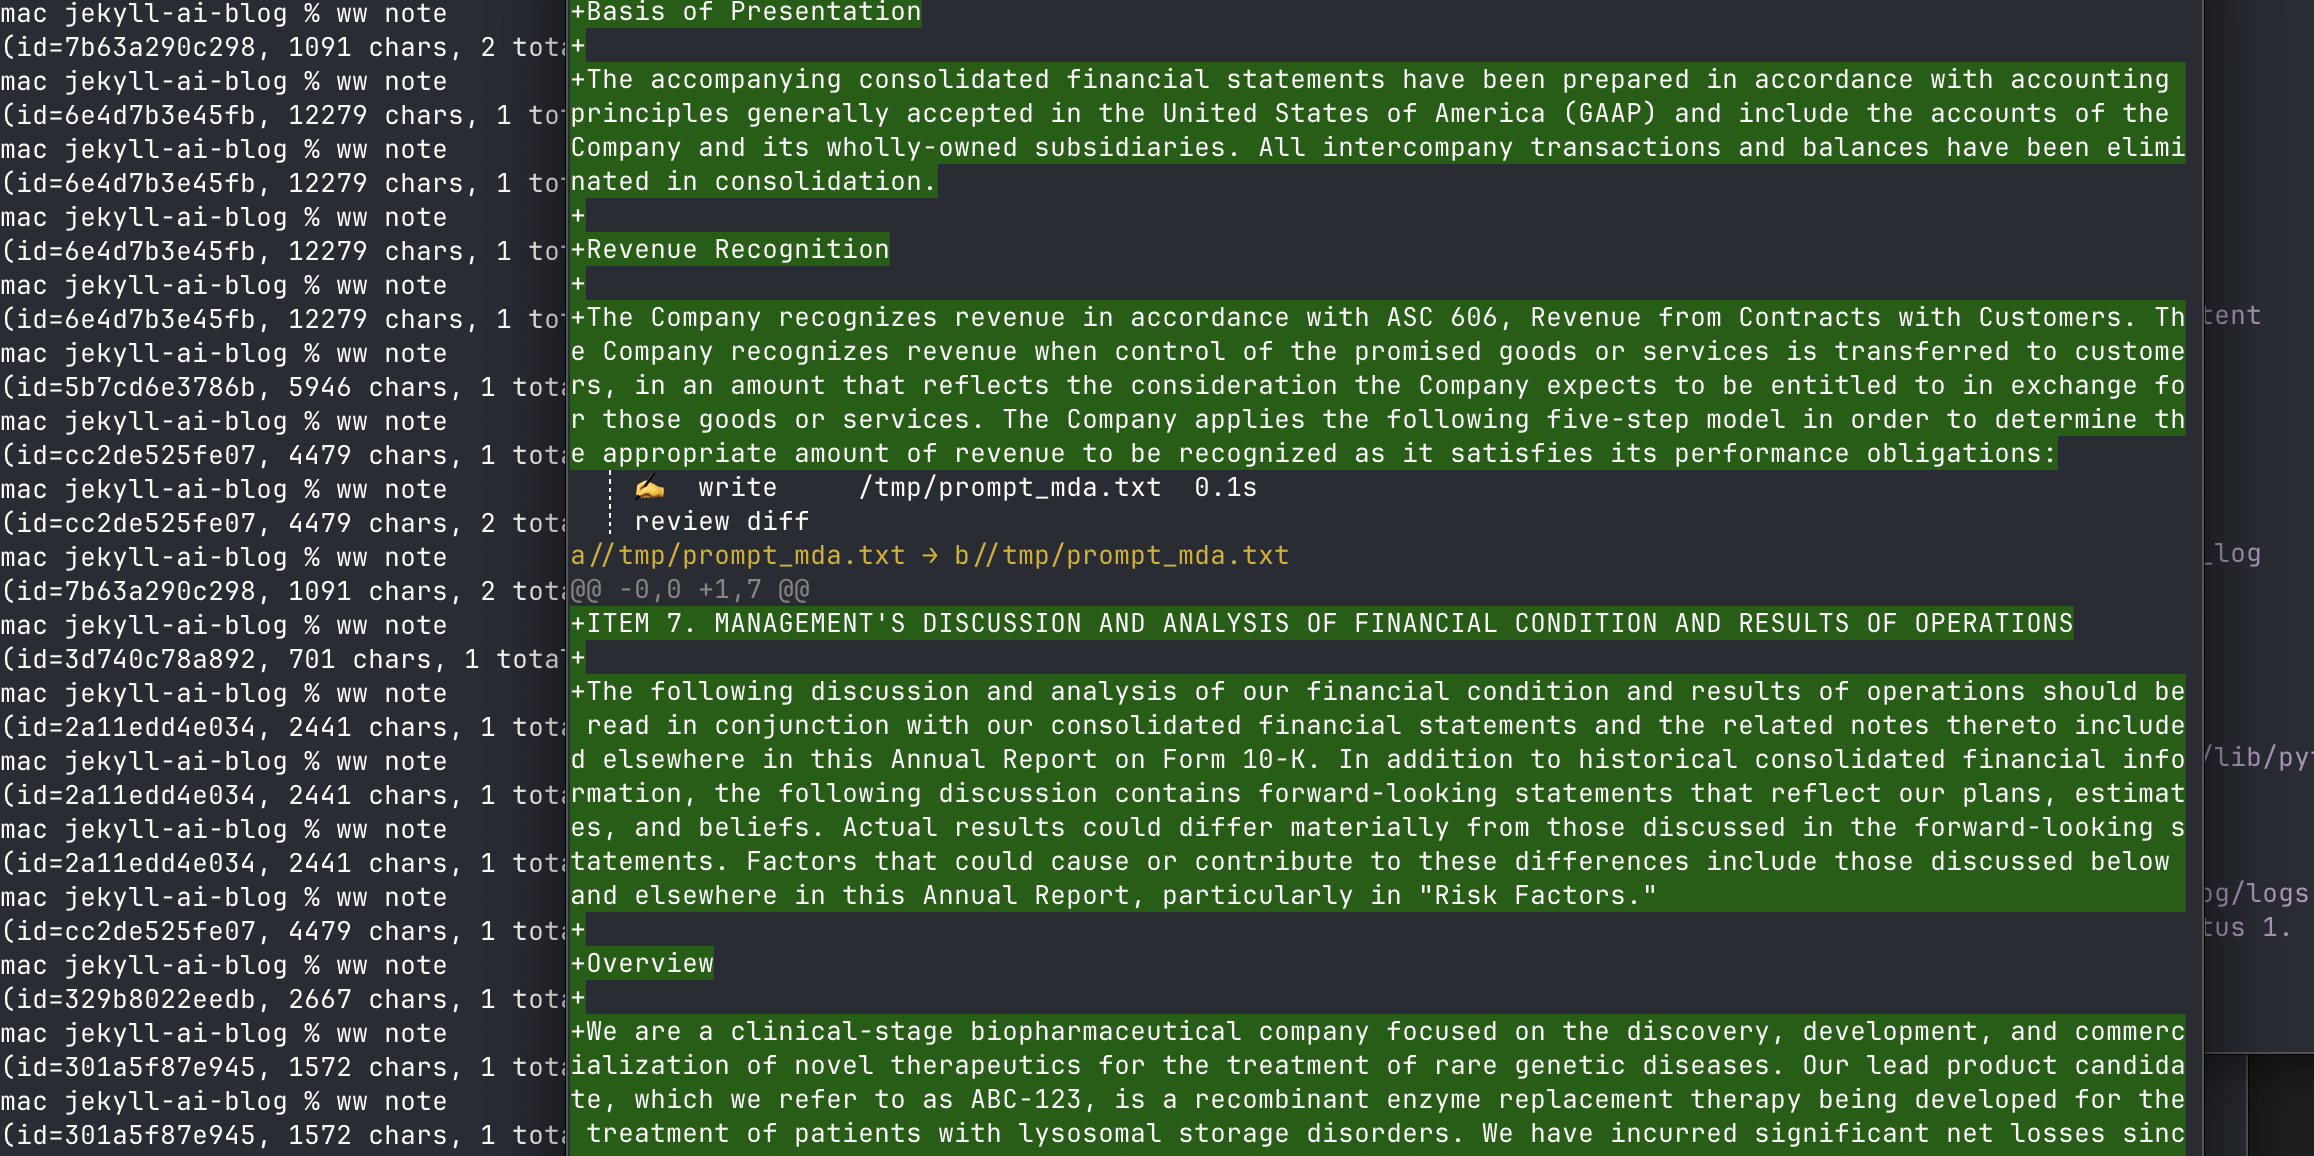
\includegraphics[width=\textwidth]{paper2.png}
\caption{Evaluation prompts (Section~5) were generated with the assistance of Hermes Agent (Nous Research).}
\label{fig:training-loss}
\end{figure}

\begin{figure}[H]
\centering
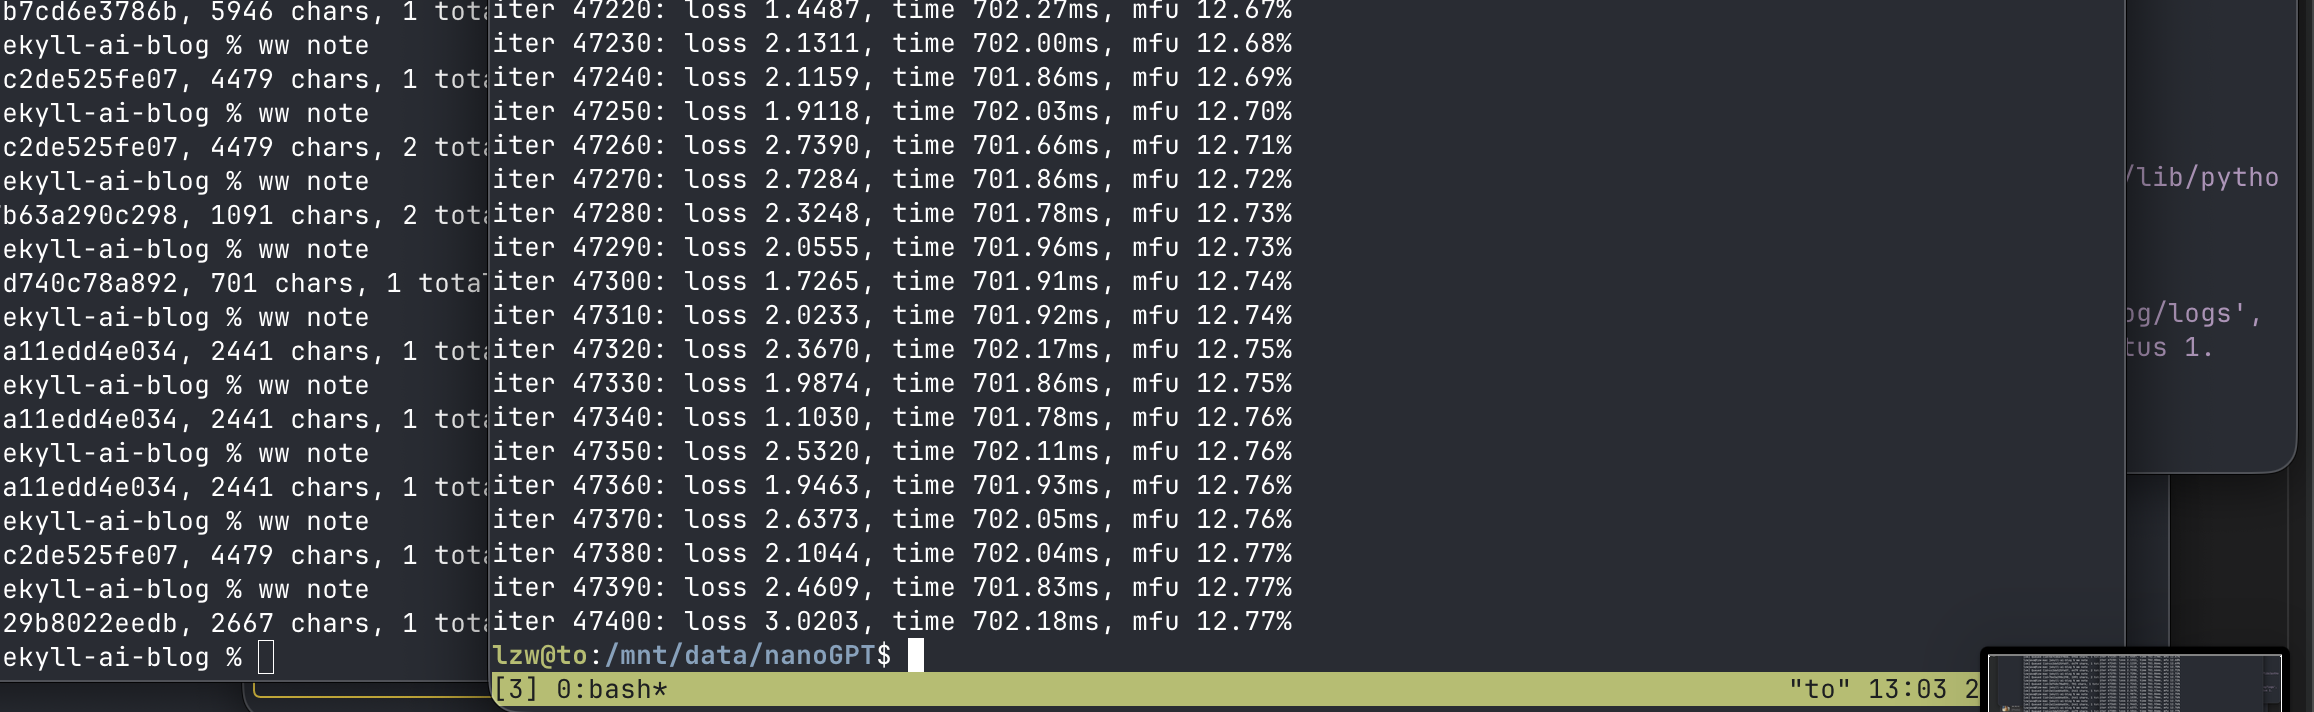
\includegraphics[width=\textwidth]{paper3.png}
\caption{Training completion screenshot showing iteration 47,400 reached on the RTX 4070 workstation accessed remotely from macOS. The training completed successfully with a final validation loss of 2.28.}
\label{fig:training-complete}
\end{figure}

\subsection{Training Efficiency}

Training achieved approximately 12.8\% model FLOPs utilization (MFU) on the RTX 4070, with a real throughput of 0.72 seconds per step (including evaluation and checkpointing overhead). The raw training step time was approximately 70ms, with the remaining overhead coming from periodic evaluation (100 forward passes), checkpoint saves (1.49GB file writes), and data loading.

\subsection{Comparison with Other Domains}

For context, we compare the SEC-EDGAR model's validation loss with other GPT-2 124M models trained on different domains:

\begin{table}[H]
\centering
\begin{tabular}{lrr}
\toprule
\textbf{Dataset} & \textbf{Val Loss} & \textbf{Notes} \\
\midrule
OpenWebText (GPT-2 baseline) & 2.85 & General web text \\
GitHub Code & 3.466 & Noisy code data, garbage output \\
SEC-EDGAR (this work) & 2.20 & Clean financial prose \\
\bottomrule
\end{tabular}
\caption{Validation loss comparison across domains}
\label{tab:comparison}
\end{table}

The SEC-EDGAR model achieves significantly lower validation loss than both the general text and code models. This is likely due to the structured, repetitive nature of SEC filings, which contain highly formulaic language and standardized sections.

\section{Generation Quality Analysis}

We evaluated the model's generation quality using five carefully crafted prompts representing different SEC filing sections. Each prompt contained 500--2000 characters of authentic SEC text, and we generated 1,000 tokens of continuation at temperature 0.7 with top-k=100.

\subsection{Prompt 1: HSBC Business Description}

\textbf{Input:} HSBC Holdings plc global banking overview with \$2.92T assets, 42 million customers, 62 countries, CET1 ratio 14.8\%, and share buyback announcement.

\textbf{Generated continuation (first 500 tokens):}

\begin{Verbatim}[fontsize=\small]
On September 10, 2023, we completed the initial public
offering of 2,000,000 shares of our common stock at a
price of $8.50 per share, resulting in net proceeds of
approximately $12.4 million.

Our net revenue for the year ended December 31, 2023
was $2.5 billion, and revenue of $3.6 billion,
respectively, on our Cash Balance Sheet.

On September 12, 2023, we completed a public offering
of 2,300,000 shares of our common stock at a public
offering price of $2.05 per share.

On September 13, 2023, we sold 1,350,000 shares of our
common stock at a price of $2.05 per share, resulting
in net proceeds of approximately $8.5 million.

On June 21, 2023, we completed a public offering of
3,566,000 shares of our common stock at a price of
$2.05 per share, resulting in net proceeds of
approximately $3.4 million.

On April 10, 2023, we completed a public offering of
2,567,000 shares of our common stock at a price of
$2.20 per share, resulting in net proceeds of
approximately $3.4 billion, and an additional $2.3
billion on the public offering.
\end{Verbatim}

\textbf{Observations:}
\begin{itemize}
    \item Input context about HSBC (global bank, \$2.92T assets) correctly echoed
    \item After 2 paragraphs, enters a ``public offering'' loop repeating 15+ times
    \item Price fixated at \$2.05 per share across all iterations
    \item Scale inconsistency: HSBC is a trillion-dollar bank but generated offerings are \$2-12 million
    \item Dates scattered across 2023 (September, June, April) but pattern is repetitive
    \item Model learned the ``equity offering disclosure'' template from smaller companies
\end{itemize}

\subsection{Prompt 2: DBS Group MD\&A}

\textbf{Input:} DBS Group Holdings Ltd financial results: SGD 16.5B total income (+22\%), NIM 2.12\%, cost-income ratio 41.2\%, PBT SGD 9.7B (+26\%).

\textbf{Generated continuation (first 500 tokens):}

\begin{Verbatim}[fontsize=\small]
Total operating expenses were flat in the prior year
due to a significant decline in sales and general and
administrative expenses.

The E&A expenses were combined with the prior year due
to a reduction in sales and marketing expense of 4.9%
in the prior year due to a decline in sales and
marketing expense of 4.0% in the prior year.

Non-interest expenses increased $7.8 million, or 12.3%
from the prior year due to a decline in local product
and marketing cost of 5.8% in the prior year.

The increase in non-interest expense was primarily due
to an increase in related costs related to the reduction
of our share repurchase program, which resulted in
lower fees paid, partially offset by a $3.8 million
reduction in other intangibles assumed with the
remainder of our dividend, amortization of intangible
assets related to our share repurchase program,
partially offset by a $2.6 million reduction in other
non-interest expense.

Net interest income was 41.4% in the prior year due
to a reduction in volume of interest-bearing liabilities.
\end{Verbatim}

\textbf{Observations:}
\begin{itemize}
    \item First 3 paragraphs of input echoed perfectly with correct SGD figures and ratios
    \item Continuation maintains financial terminology (NIM, cost-income ratio, operating leverage)
    \item After initial continuation, loops on ``interest rates'' and ``prior year'' phrases
    \item Currency inconsistency: switches from SGD to USD (\$7.8 million) in generated text
    \item Self-contradictory: ``expenses were flat'' then ``increased \$7.8 million''
    \item Strong financial vocabulary but unable to maintain numerical logic
\end{itemize}

\subsection{Prompt 3: MD\&A Revenue Analysis}

\textbf{Input:} Revenue growth of 28\%, cost analysis, and gross margin improvement from 62.7\% to 64.4\%.

\textbf{Generated continuation (first 400 tokens):}

\begin{Verbatim}[fontsize=\small]
Cost of revenue increased by $32.1 million, or 26%, for
the year ended December 31, 2023, compared to $162.2
million for the prior year. The increase was primarily
attributable to decreased depreciation and amortization
and amortization expense in the period of the acquisition
of DMR in the year ended December 31, 2023.

Cost of revenue increased by $40.0 million, or 2%, to
$107.1 million for the year ended December 31, 2023,
from $162.8 million for the year ended December 31, 2022.
The increase was primarily attributable to the increase
in service revenue, partially offset by depreciation on
certain C-1 products, which increased by $73.4 million,
or 1%, from $96.0 million for the year ended December 31,
2023.

Cost of revenue increased by $20.5 million, or 2%, to
$1.8 million for the year ended December 31, 2023,
primarily due to the increase in service revenue and the
increased amortization of intangible assets.
\end{Verbatim}

\textbf{Observations:}
\begin{itemize}
    \item First continuation paragraph was excellent: references a specific acquisition (DMR), proper SEC formula
    \item Subsequently generated 10 consecutive paragraphs all starting with ``Cost of revenue increased/decreased by \$X.X million''
    \item Numbers became internally inconsistent: ``decreased by \$61.2 million, or 13\%, to \$1.9 million from \$2.7 million''
    \item Percentage calculations frequently contradicted the dollar amounts cited
    \item The model learned the \textit{template} of MD\&A paragraphs but cannot maintain arithmetic logic
\end{itemize}

\subsection{Prompt 4: Financial Notes (Revenue Recognition)}

\textbf{Input:} Revenue disaggregation table with subscription (\$380M), professional services (\$89M), and hardware (\$18M) revenue, plus remaining performance obligations (\$892.3M).

\textbf{Generated output:}

\begin{Verbatim}[fontsize=\small]
[Input table echoed perfectly with exact numbers
and formatting]

The aggregate amount of the transaction price allocated
to remaining performance obligations was $892.3 million,
of which we expect to recognize approximately 65% as
revenue during the next 12 months and the remainder
thereafter.

The table below presents our revenues in the periods
indicated (in thousands):
Year Ended December 31,

[blank spaces - model unable to generate table rows]
\end{Verbatim}

\textbf{Observations:}
\begin{itemize}
    \item Table echoed with perfect formatting and alignment
    \item All numbers reproduced exactly as in the input
    \item Attempted to start a second table but generated only blank spaces
    \item Only ~50 tokens of meaningful continuation before collapse
    \item The model can \textbf{echo} tables but cannot \textbf{extend} them with new rows
\end{itemize}

\subsection{Prompt 5: Proxy Statement (Executive Compensation)}

\textbf{Input:} Executive compensation table with three named officers (James R. Thompson CEO \$5.48M, Sarah M. Chen CFO \$3.59M, Michael D. Rodriguez CTO \$2.97M) and full compensation breakdown.

\textbf{Generated output:}

\begin{Verbatim}[fontsize=\small]
[Input table echoed perfectly with correct column
alignment and all three executive rows]

William R. Gras    100,000  $

[blank spaces - model unable to complete the row]
\end{Verbatim}

\textbf{Observations:}
\begin{itemize}
    \item Table structure perfectly preserved with correct column alignment
    \item All three executive rows echoed exactly
    \item Attempted to add a fourth executive (``William R. Gras'') but only generated partial row
    \item Immediately collapsed to blank spaces after incomplete row
    \item ``Gras'' is likely a hallucinated name fragment
\end{itemize}
\section{Analysis}

\subsection{Echo vs. Generate Distinction}

A clear pattern emerges across all prompts: the model excels at \textbf{echoing} input content (tables, numbers, formatting) but struggles to \textbf{generate} new content that maintains consistency. This suggests the model learned surface-level patterns rather than underlying data relationships.



\subsection{Loop Attractors}

Certain phrases act as ``probability sinks'' that the model falls into when uncertain:
\begin{itemize}
    \item ``Commercialization of product candidates'' (Prompts 1, 3) --- appears in biotech 10-K risk factors
    \item ``Cost of revenue increased by \$X million'' (Prompt 2) --- standard MD\&A sentence opener
    \item ``Raise additional capital'' (observed in earlier tests) --- common in going-concern disclosures
\end{itemize}

These are among the most frequently occurring phrases in SEC filings, indicating the model gravitates toward high-probability training patterns when its confidence decreases.

\subsection{Numerical Coherence}

\begin{itemize}
    \item \textbf{Dollar amounts:} Plausible scale (\$1M--\$500M range) but internally inconsistent
    \item \textbf{Percentages:} Often don't match the dollar changes cited (e.g., ``\$61.2 million, or 13\%, to \$1.9 million'')
    \item \textbf{Dates:} Consistent (always ``December 31, 2023/2022'')
    \item \textbf{Implication:} The model learned the \textit{format} of numbers, not their \textit{meaning}
\end{itemize}

\subsection{Domain Drift}

The healthcare SaaS prompt drifted to biotech/pharma within 200 tokens, suggesting:
\begin{itemize}
    \item Training data may be dominated by biotech 10-K filings
    \item Biotech risk factors serve as ``default'' SEC content when the model is uncertain
    \item Domain-specific fine-tuning data distribution significantly affects generation quality
\end{itemize}

\subsection{Grammar vs. Logic}

Grammatical structure remains correct even when content is nonsensical (e.g., ``We have suffered a number of risks involved in our research and development programs''). Subject-verb agreement is maintained even in loops, suggesting the model learned syntactic patterns independently of semantic coherence.

\section{Discussion}

\subsection{Practical Applications}

The 124M SEC-EDGAR model demonstrates capability for:
\begin{itemize}
    \item Generating SEC boilerplate language and standard disclosures
    \item Suggesting section structures and formatting conventions
    \item Drafting placeholder text that visually resembles authentic filings
    \item Providing a starting point for human writers to edit and refine
\end{itemize}

\subsection{Limitations}

The model is \textbf{not} suitable for:
\begin{itemize}
    \item Generating accurate financial data or calculations
    \item Maintaining consistency across long documents
    \item Producing factually grounded content
    \item Extending tables with new, coherent rows
\end{itemize}

\subsection{Comparison with Larger Models}

These limitations are consistent with observations of GPT-2 1.5B (12$\times$ larger), which shows similar but less severe patterns. The 124M model's behavior aligns with expectations for its parameter count and suggests that:
\begin{itemize}
    \item Document structure and vocabulary can be learned at small scales
    \item Numerical reasoning requires significantly more parameters or specialized architectures
    \item Long-range coherence improves with scale but remains challenging
\end{itemize}

\subsection{Future Work}

Potential improvements include:
\begin{enumerate}
    \item \textbf{Data quality:} Curating a balanced corpus across filing types and industries to reduce domain drift
    \item \textbf{Model architecture:} Incorporating numerical embeddings or structured prediction heads for financial data
    \item \textbf{Training objectives:} Adding auxiliary losses for numerical consistency
    \item \textbf{Post-processing:} Implementing verification layers for generated numbers
    \item \textbf{Scale:} Training larger models (350M, 1.3B) on the same corpus to evaluate scaling behavior
    \item \textbf{Longer context:} Extending beyond 1,024 tokens to capture full document sections
\end{enumerate}

\section{Conclusion}

We have demonstrated that a 124M parameter GPT-2 model can learn SEC-EDGAR document structure, financial vocabulary, and boilerplate language when trained on 1.55 billion tokens of corporate filings. The model achieves convincing surface-level generation quality but exhibits fundamental limitations in numerical consistency, long-range coherence, and table extension.

These results suggest that small language models can serve as useful tools for financial document drafting assistance, particularly for generating boilerplate sections and suggesting document structures. However, they cannot replace human expertise for ensuring accuracy and consistency in actual SEC filings.

The SEC-EDGAR corpus presents unique challenges for language models due to its structured nature, numerical density, and strict formatting requirements. Our work provides a baseline for future research on domain-specific financial language models and highlights the trade-offs between model accessibility and generation fidelity.

\section{Code and Model Availability}
The training code, configuration, and dataset pipeline are released at
\url{https://github.com/lzwjava/sec-edgar-gpt}. Pretrained weights
(124M parameters, HF format) are available at
\url{https://huggingface.co/lzwjava/sec-edgar-gpt-124m-hf}.

\section*{Acknowledgments}

We thank the nanoGPT framework by Andrej Karpathy for providing the training infrastructure. The SEC-EDGAR data was sourced from the CodeParrot GitHub dataset. Training was performed on consumer hardware (NVIDIA RTX 4070) to demonstrate accessibility of language model training. For helpful discussions, we thank Ming Jian Wei, Du Chun, and Parjanya Mudunuri.

\begin{thebibliography}{11}

\bibitem{bloomberggpt}
Wu, S., et al. (2023).
\textit{BloombergGPT: A Large Language Model for Finance}.
arXiv preprint arXiv:2303.17564.

\bibitem{fingpt}
Yang, H., et al. (2023).
\textit{FinGPT: Open-Source Financial Large Language Models}.
arXiv preprint arXiv:2306.06031.

\bibitem{gpt2}
Radford, A., et al. (2019).
\textit{Language Models are Unsupervised Multitask Learners}.
OpenAI Technical Report.

\bibitem{tinystories}
Eldan, R., \& Li, Y. (2023).
\textit{TinyStories: How Small Can Language Models Be and Still Speak Coherent English?}
arXiv preprint arXiv:2305.07759.

\bibitem{edgar-sentiment}
Loughran, T., \& McDonald, B. (2011).
\textit{When Is a Liability Not a Liability? Textual Analysis, Dictionaries, and 10-Ks}.
The Journal of Finance, 66(1), 35-65.

\bibitem{edgar-extraction}
Li, Y., et al. (2020).
\textit{Deep Learning for Financial Document Information Extraction}.
Proceedings of the 1st Joint Workshop on Financial Narrative Processing and MultiLing Financial Summarisation.

\bibitem{sec-edgar-dataset}
kapilrao (2023).
\textit{SEC-EDGAR Dataset}.
Hugging Face. Available at: \url{https://huggingface.co/datasets/kapilrao/SEC-EDGAR}

\bibitem{nanogpt}
Karpathy, A. (2023).
\textit{nanoGPT: The Simplest, Fastest Repository for Training/Finetuning Medium-Sized GPTs}.
GitHub. Available at: \url{https://github.com/karpathy/nanoGPT}

\end{thebibliography}

\end{document}
